Auch die verwendeten Tools haben einen entscheidenden Einfluss auf unser Projekt gehabt.
Deshalb sind im Folgenden die wichtigsten 3 dargestellt.


\subsection{Git --- Versionskontrolle}\label{subsec:git-----versionskontrolle}
Git ist ein Versionierungssystem, das textbasiert Änderungen erkennen und verwalten kann.
Dies bietet insofern einen Vorteil in diesem Projekt gegenüber Alternativen, wie Bitbucket, die nicht auf Textebene arbeiten, dass zeichenweise Änderungen erkannt und zusammengeführt werden können.
Sofern Änderungen in verschiedenen Zeilen sind, meist sogar automatisch.


Diese Änderungen sind dabei in Commits unterteilt.
So können wir unbeirrt entwickeln, ohne uns Sorgen machen zu müssen, ob wir etwas Falsches löschen.


Auch können wir so mit der Platform \href{https://github.com/WHS-SLAB-WiSe22-23-P1/Labyrinth}{GitHub} kollaborieren.
Dies ist in den folgenden beiden Abschnitten~\ref{subsubsec:git--flow-----branching} und~\ref{subsubsec:conventional-commits} genauer dargestellt.

\subsubsection{Git--Flow --- Branching}\label{subsubsec:git--flow-----branching}
\begin{figure}
    \centering
    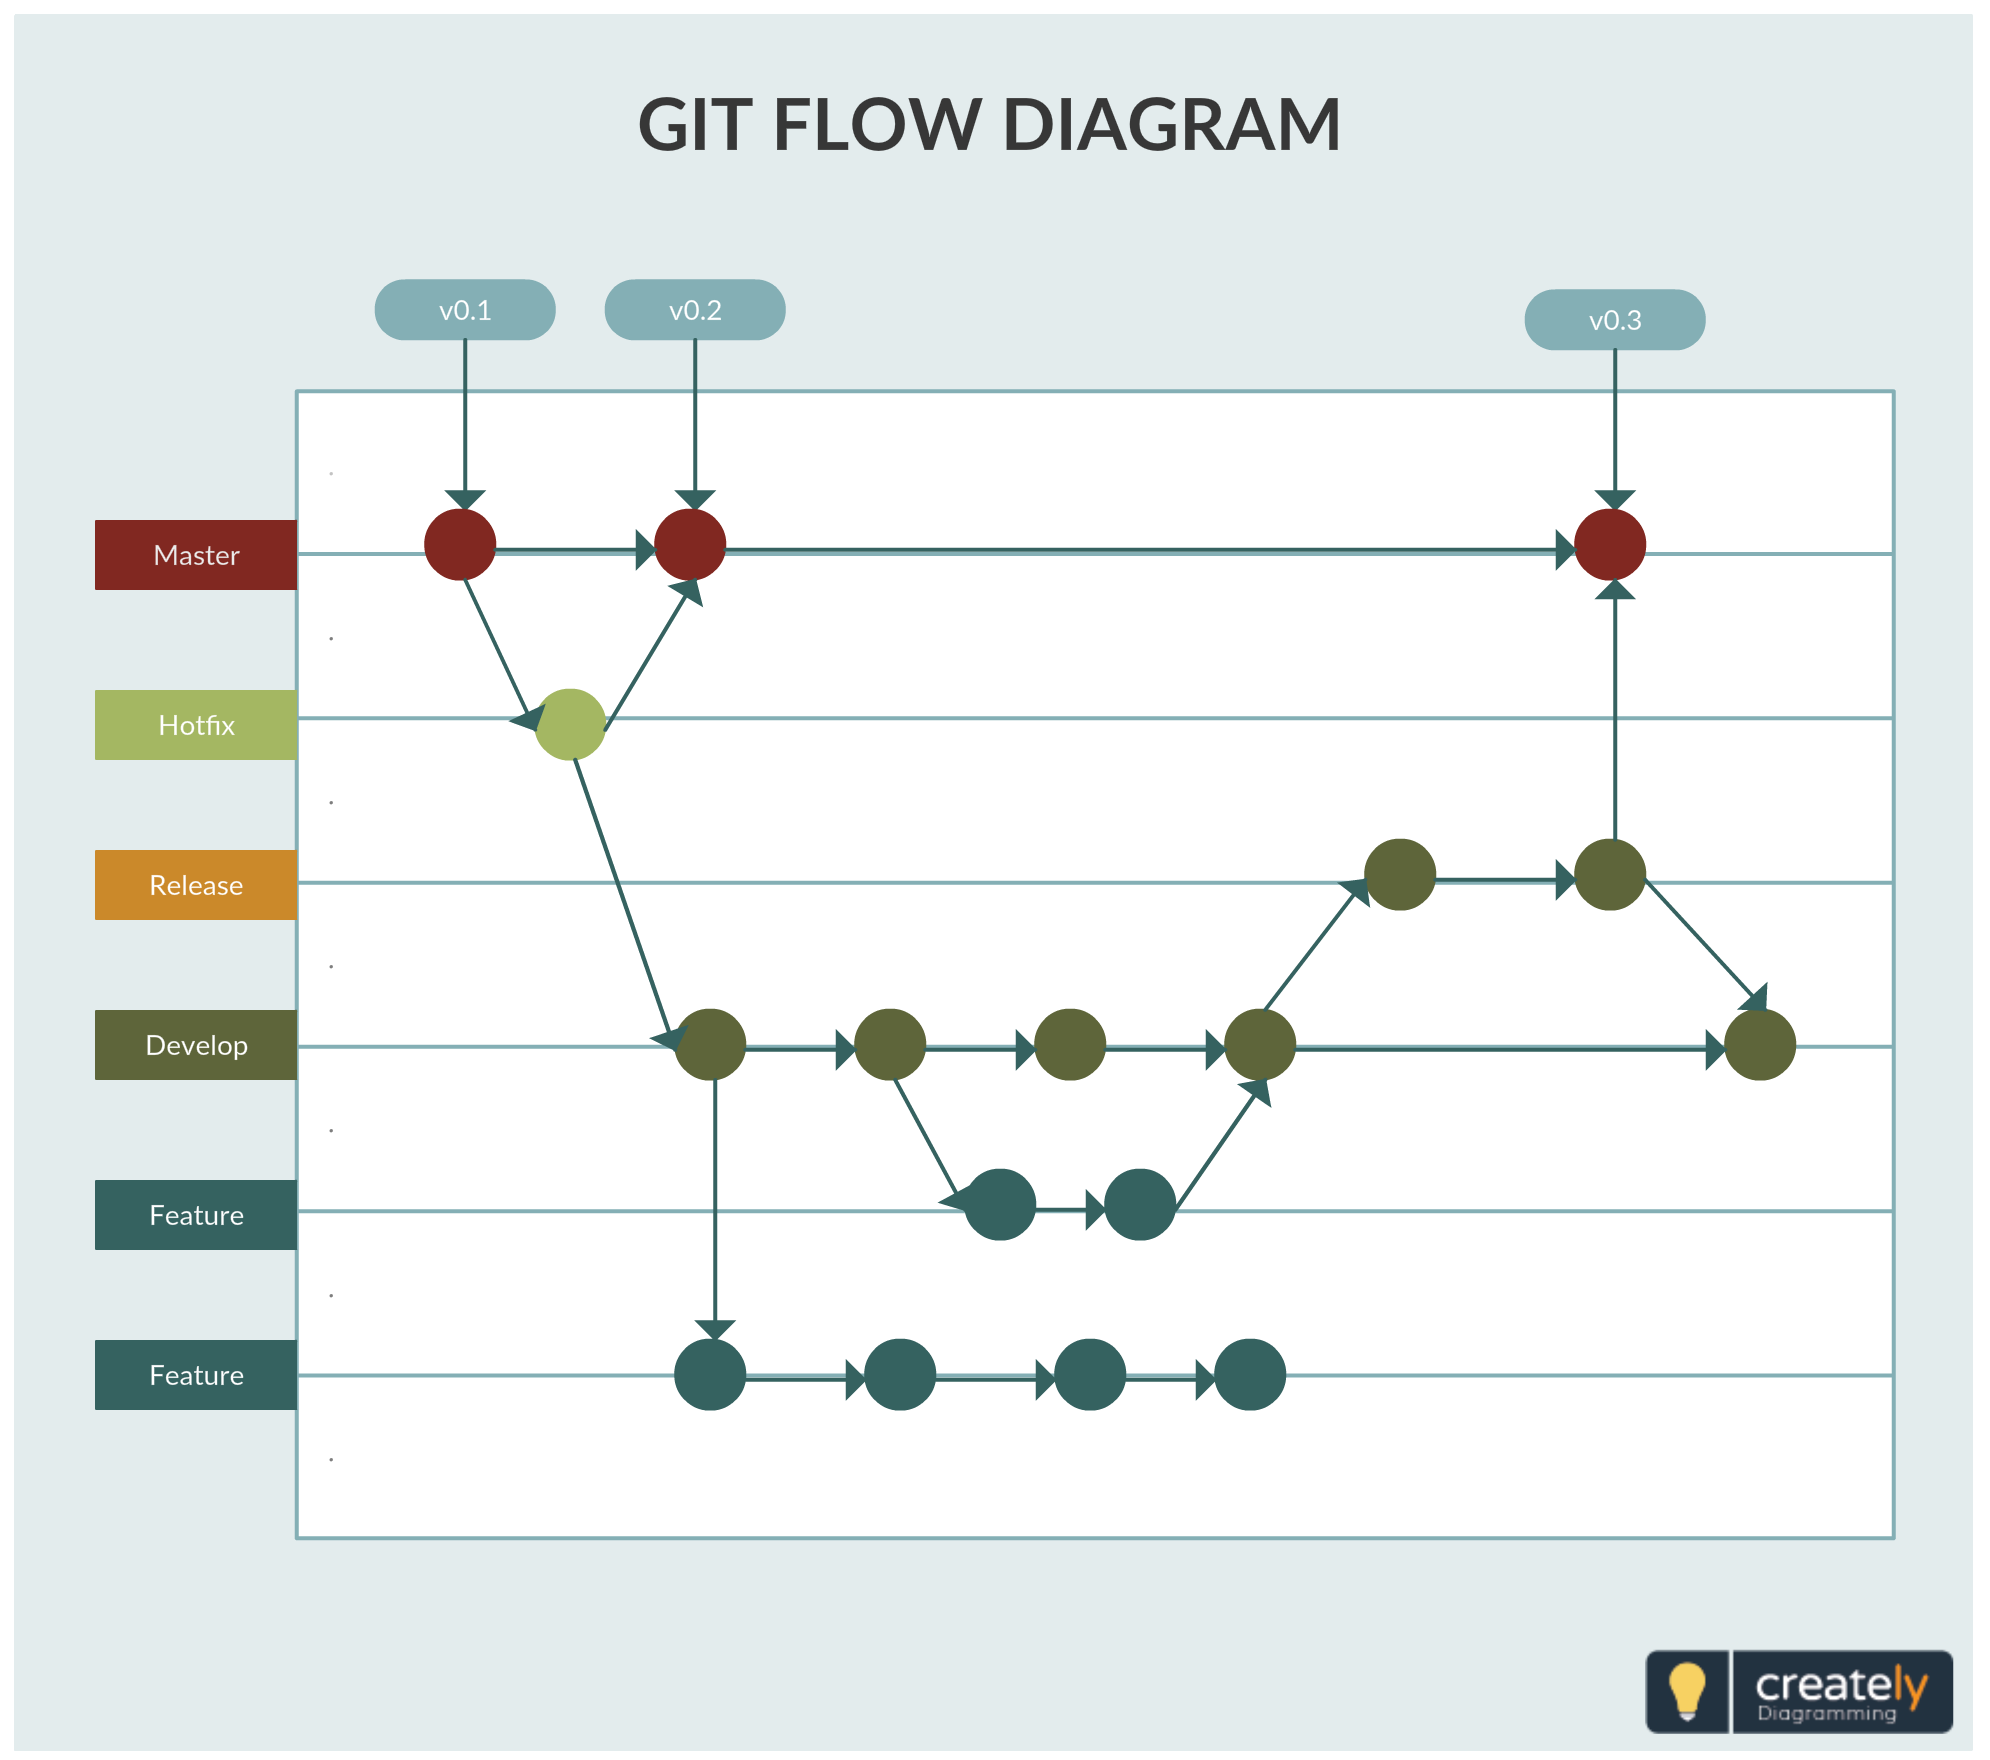
\includegraphics[width=\paperwidth-2in]{../assets/img/git_flow}
    \caption{Branches im Git--Flow Modell~\autocite{creately-no-date}}
    \label{fig:git-flow}
\end{figure}
Branching ist eines der wichtigsten Konzepte der Versionskontrolle.
Es erlaubt mehreren Entwicklern gleichzeitig an verschiedenen Features zu arbeiten.
Ein Branch ist dabei ein Pointer auf einen Commit.
Werden zwei Branches zusammengeführt, so sprechen wir von einem Merge.
Git-Flow ist ein Modell, wie Branches angelegt und strukturiert werden sowie was wohin gemerged wird.


\paragraph{Main} (In Abbildung~\ref{fig:git-flow} Master genannt) beschreibt dabei die aktuelle Release--Version.
Es wird niemals direkt in \textbf{Main} committed.


\paragraph{Develop} ist die aktuelle Entwicklungs--Version.
Hier wird getestet, ob \textbf{Features} gut zusammen funktionieren, also keine semantischen Fehler durch einen Merge aufgetreten sind.
Es dürfen nur Commits erstellt werden, die einen solchen Fehler beheben.


\paragraph{Features} sind nicht zwangsläufig neue Features.
Es kann sich dabei auch um einen Bugfix oder Dokumentation, etc.\ handeln.
In einem \textbf{Feature} arbeitet nur ein Entwickler zur selben Zeit.
Features haben \textbf{Develop} als Upstream und werden nach fertigstellung in \textbf{Develop} gemerged.


\paragraph{Hotfixes} sollen kritische Bugs schnell fixen.
Es sind \textit{Shortcut Features}, die mit upstream \textbf{Main} direkt wieder in \textbf{Main} gemerged werden.
Anschließend wird \textbf{Main} in \textbf{Develop} gemerged, damit alle wieder mit dem aktuellsten Stand arbeiten.


\paragraph{Releases} haben \textbf{Develop} als Upstream und werden in \textbf{Main} gemerged.
Sie sind für die Release--Vorbereitung gedacht.
Hier wird zum Beispiel die Version angepasst oder mit Conventional Commits~\ref{subsubsec:conventional-commits} ein Changelog generiert.
Nach dem Release wird \textbf{Main} in \textbf{Develop} gemerged.


\paragraph Wir nutzen eine etwas abgespeckte Version ohne \textbf{Release}-- sowie \textbf{Hotfix}--Branches, da wir keine Releaseversion verwalten müssen.


\subsubsection{Conventional Commits}\label{subsubsec:conventional-commits}
Mit dieser, ursprünglich für das Web--Framework Angular entwickelten Konvention lassen sich git leserliche sowie leicht zu parsende Commit Nachrichten verfassen.
Sie entsprechen dem Format \qq{<feat|fix|build|chore|ci|docs|style|refactor|perf|test>(<scope>): <message>}.


Die Änderungen sind zunächst in eine der \textbf{Kategorien} zu unterteilen.
Bei komplexen Projektspezifikationen können auch andere als die aufgeführten auf Projektebene spezifiziert werden.


Anschließend kann ein \textbf{Scope} angegeben werden.
Dies bietet sich vor allem bei einem Monorepo bzw.\ Multi--Module--Setup, wie unserem an.
Unsere \textbf{Scopes} entsprechen dem bearbeiteten Maven~\ref{subsec:maven-----build--management} Modulen.
Lässt sich kein eindeutiges \textbf{Scope} bestimmen, oder ist das Projekt zu klein, wird das \textbf{Scope} ausgelassen.


Die \textbf{Nachricht} beschreibt, was geändert wurde.
Sie sollte so formuliert werden, dass das thema der Änderung in wenigen Worten verständlich ist.


Das Format muss nicht in Feature--Branches verwendet werden, wenn diese gesquashed (komprimiert) werden.
Es sollte aber bei allen Commits, die in Develop landen angewendet werden.
Daraus können dann sehr einfach Changelogs und ähnliches generiert werden.


\subsection{Maven --- Build--Management}\label{subsec:maven-----build--management}
Mit Maven lässt sich der Aufbau des Projekts beschreiben.


Zum einen müssen die Abhängigkeiten (Dependencies) lediglich als eine URI angegeben werden.
So muss sich nicht jeder dieselben JARs herunterladen und in der IDE~\ref{subsec:intellij-----ide} manuell einbinden.


Aber auch lässt sich die Software in Module unterteilen.
So muss nicht alles in dieselbe JAR komprimiert werden und Front-- und Backend können im selben Repository arbeiten.
Aber auch gemeinsame Abhängigkeiten, wie unser Datenmodell, lassen sich damit erstellen.


Alles in allem kümmert sich das Tool darum, dass alle nötigen Module in der richtigen Reihenfolge kompiliert und zusammengefügt werden.


Ein großes Problem war es, dass die neuste major Version von Processing nicht mit Maven veröffentlicht wurde.
Wir haben also ein Kompilat des öffentlichen Repositories eines Drittanbieters genutzt.
Damit hatten wir allerdings lediglich die Core Library zur Verfügung.


\subsection{IntelliJ --- IDE}\label{subsec:intellij-----ide}
Mittels Maven~\ref{subsec:maven-----build--management} war eis ein leichtes, Processing in dieser \textit{\textbf{I}ntegrated \textbf{D}evelopment \textbf{E}nvironment} einzubinden.
Dies bietet uns den Vorteil einiger Unterstützung, die die Processing IDE nicht bieten kann.
So ist das Syntax-highlighting und der Autocomplete durch IntelliSense hervorragend.
Auch die Maven Struktur war in wenigen Minuten erstellt.
Auch ließ sich diese \LaTeX Dokumentation mit einem Plugin mit derselben Unterstützung generieren.
Es hat uns insgesamt sehr viel Zeit erspart, da wir vieles nicht manuell machen mussten.
\qq{Ein Entwickler, der nicht in seiner IDE lebt, ist kein guter Entwickler} --- Oder zumindest so ähnlich.